%! Suppress = MissingImport
%%
%% sample document for AAMAS'19 conference
%%
%% modified from sample-sigconf.tex
%%
%% see ACM instructions acmguide.pdf
%%
%% AAMAS-specific questions? F.A.Oliehoek@tudelft.nl
%%

\pdfminorversion=7  % Fixes .eps image files

\documentclass[sigconf]{aamas}  % do not change this line!
%% your usepackages here, for example:
\usepackage{booktabs}
\usepackage{listings}
\usepackage{graphicx}
\usepackage{float}
\usepackage{algorithm}
\usepackage{algorithmic}
\usepackage{appendix}
\usepackage{soul}
\usepackage[]{todonotes}

%% do not change the following lines
\setcopyright{ifaamas}  % do not change this line!
\acmDOI{doi}  % do noadat change this line!
\acmISBN{}  % do not change this line!
\acmConference[AAMAS'20]{Proc.\@ of the 19th International Conference on Autonomous Agents and Multiagent Systems (AAMAS 2020), B.~An, N.~Yorke-Smith, A.~El~Fallah~Seghrouchni, G.~Sukthankar (eds.)}{May 2020}{Auckland, New Zealand}  % do not change this line!
\acmYear{2020}  % do not change this line!
\copyrightyear{2020}  % do not change this line!
\acmPrice{}  % do not change this line!


%% the rest of your preamble here
\lstset{
  basicstyle=\ttfamily,
  columns=fullflexible,
  frame=single,
  breaklines=true,
  postbreak=\mbox{\textcolor{red}{$\hookrightarrow$}\space},
  basicstyle=\small,
}

%%%%%%%%%%%%%%%%%%%%%%%%%%%%%%%%%%%%%%%%%%%%%%%%%%%%%%%%%%%%%%%%%%%%%%%%%%%%%%%%%%%%%%%%%%%%%%%%%%%%%%%%%

\begin{document}

\title{Auction-based Mechanisms for Allocating Elastic Resources in Edge Clouds} 
%\titlenote{Produces the permission block, and copyright information}

% AAMAS: as appropriate, uncomment one subtitle line; check the CFP
%\subtitle{Extended Abstract}
%\subtitle{Industrial Applications Track}
%\subtitle{Socially Interactive Agents Track}
%\subtitle{Blue Sky Ideas Track}
%\subtitle{Engineering Multiagent Systems Track}
%\subtitle{Robotics Track}
%\subtitle{JAAMAS Track}
%\subtitle{Doctoral Mentoring Program}

%\subtitlenote{The full version of the author's guide is available as \texttt{acmart.pdf} document}


% AAMAS: submissions are anonymous for most tracks
\author{Paper \#XXX}  % put your paper number here!

%% example of author block for camera ready version of accepted papers: don't use for anonymous submissions
%

\begin{abstract}  % put your abstract here!
Edge clouds enable computational tasks to be completed at the edge of the network, without relying on access to remote data centres. A key challenge in these settings is that limited computational resources often need to be allocated to many self-interested users. Here, existing resource allocation approaches usually assume that tasks have inelastic resource requirements (i.e., a fixed amount of compute time, bandwidth and storage), which may result in inefficient resource use. To address this, we propose a novel approach that takes advantage of the elastic nature of some of the resources, e.g., to trade off computation speed with bandwidth if this allows a server to execute more tasks by their deadlines. We describe this problem formally, show that it is NP-hard and then propose a scalable approximation algorithm. To deal with the self-interested nature of users, we show how to design a centralized auction that incentivizes truthful reporting of task requirements and values. Moreover, we propose  novel auction-based decentralized approaches that are not always truthful, but that limit the information required from users and that can be adjusted to trade off convergence speed with solution quality. In extensive simulations, we show that considering the elasticity of resources leads to a gain in utility of around \hl{XX\%} compared to existing fixed approaches and that our novel auction-based approaches typically achieve \hl{YY-ZZ\%} of the theoretical optimal.
%With the rise of fog cloud computing, resource allocation is ever more important as server encounter bottlenecks
%(e.g. CPU cycles, memory and bandwidth) due to their limited capacity. 
%In this paper, we introduce flexible resource allocation mechanisms where the server chooses the amount of
%resources allocated to each task compared to a task requesting a fixed quantity of resources.
%We propose four algorithms. two novel, a greedy algorithm to maximise social welfare and three auction mechanisms: 
%a single-domain parameter auction where users must reveal their reserve price, a novel evolutionary pricing 
%mechanism as well as a novel decentralised iterative auction that uses a reverse VCG mechanism to determine the prices.
%Extensive simulation results show that our algorithms outperform current fixed approaches and is very close to the optimal.
\end{abstract}


% AAMAS: the ACM CCS are not needed within AAMAS papers
%%
%% The code below should be generated by the tool at
%% http://dl.acm.org/ccs.cfm
%% Please copy and paste the code instead of the example below.
%%
%\begin{CCSXML}
%<ccs2012>
% <concept>
%  <concept_id>10010520.10010553.10010562</concept_id>
%  <concept_desc>Computer systems organization~Embedded systems</concept_desc>
%  <concept_significance>500</concept_significance>
% </concept>
% <concept>
%  <concept_id>10010520.10010575.10010755</concept_id>
%  <concept_desc>Computer systems organization~Redundancy</concept_desc>
%  <concept_significance>300</concept_significance>
% </concept>
% <concept>
%  <concept_id>10010520.10010553.10010554</concept_id>
%  <concept_desc>Computer systems organization~Robotics</concept_desc>
%  <concept_significance>100</concept_significance>
% </concept>
% <concept>
%  <concept_id>10003033.10003083.10003095</concept_id>
%  <concept_desc>Networks~Network reliability</concept_desc>
%  <concept_significance>100</concept_significance>
% </concept>
%</ccs2012>
%\end{CCSXML}
%
%\ccsdesc[500]{Computer systems organization~Embedded systems}
%\ccsdesc[300]{Computer systems organization~Redundancy}
%\ccsdesc{Computer systems organization~Robotics}
%\ccsdesc[100]{Networks~Network reliability}


\keywords{Edge clouds; elastic resources; auctions}  % put your semicolon-separated keywords here!

\maketitle

%% start of main body of paper

\section{Introduction}\label{sec:introduction}

In the last few years, cloud computing~\cite{cloud_cite} has become a popular solution to run data-intensive applications remotely. However, in some application domains, it is not feasible to rely a remote cloud, for example when running highly delay-sensitive and computationally-intensive tasks, or when connectivity to the cloud is intermittent. To deal with such domains, \emph{mobile edge computing}~\cite{mobile_edge_survey} has emerged as a complementary paradigm, where computational tasks are executed at the edge of mobile networks at small data-centers, known as \emph{edge clouds}.


Mobile edge computing is a key enabling technology for the Internet-of-Things (IoT) \cite{mobile_edge_IoT} and in particular applications in smart cities \cite{mobile_edge_smart} and disaster response scenarios \cite{mobile_edge_disaster}. In these applications, low-powered devices generate computational tasks and data that have to be processed quickly on local edge cloud servers. More specifically, in smart cities, these devices could be smart intersections that collect data from road-side sensors and vehicles to produce an efficient traffic light sequence to minimize waiting times \hl{REF}; or it could be CCTV cameras that analyse video feeds for suspicious behaviour, e.g., to detect a stabbing or other crime in progress \hl{REF}. In disaster response, sensor data from autonomous vehicles (including video, sonar and LIDAR) can be aggregated in real time to produce maps of a devastated area, search for potential victims and help first responders in focusing their efforts to save lives \hl{REF}.

%\emph{disaster response networks},  and 
%\emph{military tactical networks},  
%where different entities need to run tasks at the servers.
%In smart cities networks, these entities could be, for example, municipal authorities checking for the traffic conditions on different parts of the city or law enforcement looking on cameras for a suspect of a crime.   
%In tactical networks, these entities could be soldiers hunting for terrorists or navy troops in a rescue mission, generals in a command center, or 
%aircraft or drones in a surveillance mission or performing air strikes.

To accomplish these tasks, there are typically several types of resources that are needed, including communication bandwidth, computational power and data storage resources \cite{vaji_infocom}, and tasks are generally delay-sensitive, i.e., have a specific completion deadline. When accomplished, different tasks carry different values for their owners (e.g., the users of IoT devices or other stakeholders such as the police or traffic authority). This value will depend on the importance of the task, e.g., analysing current levels of air pollution may be less important than preventing a large-scale traffic jam at peak times or tracking a terrorist on the run. Given that edge clouds are often highly constrained in their resources \cite{edge_limitations}, we are interested in allocating tasks to edge cloud servers to maximize the overall social welfare achieved (i.e., the sum of all task values). This is particularly challenging, because users in edge clouds are typically self-interested and may behave strategically or may prefer not to reveal private information about their values to a central allocation mechanism \hl{(ideally some REF to justify this)}.

%and also on the fact who is asking for that task. 
%For example, a general's task is more important than that of a captain, or a task in a surveillance mission is more important than getting the air humidity in different areas. %analysis of a high-value target's surveillance is
%more important than the analysis of an army base CCTV footage far away from the battlefield.

An important shortcoming of existing work looking at resource allocation in edge clouds, e.g., \cite{vaji_infocom,Bi2019}, is that it assumes tasks have strict resource requirements --- that is, each task consumes a fixed amount of computation (CPU cycles per time), takes up a fixed amount of bandwidth to transfer data and uses up a fixed amount of storage on the server. However, in practice, edge cloud servers have some flexibility in how they allocate limited resources to each task. In more detail, to execute a task, the corresponding data and/or code first has to be transferred to the server it is assigned to, requiring some bandwidth. This then takes up storage on the server. Next, the task needs computing power from the server in terms of CPU cycles per time. Once computation is complete, the results have to be transferred back to the user, requiring further bandwidth. Now, while the the storage capacity at the server for every task is \emph{strict}, since the task cannot be run unless all the data are stored, the bandwidth allocation and the speed at which the task is run on the server are \emph{elastic}. The latter two depend on how flexible the task's deadline is, and can be adjusted  accordingly, so that more tasks can receive service simultaneously. Allocating the elastic resources optimally is the focus of this paper.      

%In order to obtain successfully the outcomes of the tasks from the servers, there are some procedures that need to be followed. 
%First, every task would require to store the corresponding data and/or code to the server it is assigned to. Then, it requires some communication bandwidth
%to send the data to the server and to get the results back at the end. Finally, the task needs computing power from the server, in terms of CPU cycles. 
%While the storage capacity at the server for every task is \emph{strict}, since the task cannot be run unless all the data are stored, the rate allocation 
%and the speed at which the task is run on the server are \emph{elastic}. The latter two depend on how flexible the task's deadline is, and can be adjusted 
%accordingly, so that more tasks can receive service simultaneously. Allocating the elastic resources optimally is the focus of this paper.      

%The key research questions that arise related to this problem are:
%\begin{itemize}
%    \item Given a set of tasks arriving from different users and with different values, which all require service simultaneously from a set of edge cloud servers, what is the optimal assignment for these tasks, so that the sum of values over all served tasks is maximized? 
%    \item How can the limited resources of a server be optimally allocated to tasks to allow as many of them to run concurrently, taking into account the elasticity of some of the resources?
%    \item How can we design allocation mechanisms that can be deployed in realistic multi-agent systems, where users may be self-interested, strategic and wish to minimize the information they reveal to an allocation mechanism.
%\end{itemize}

%\todo[inline]{If we need space, can we remove these questions? I think they should be clear from preceding text.}

%To this end, in this paper we look at a static (one-shot problem) formulation of assigning the tasks to servers and allocating
%optimally the resources (bandwidth, computation, and storage) to these tasks. Assuming that the resources are limited, there
%will be tasks that cannot be served. Also, there is a deadline associated with every task, which if not met, would be the same as if not serving the task at all. So, the idea is to decide on which tasks to serve, to which server they are to be assigned and what amount of the resources they need to get, in order
%to maximize the sum of the values over all the tasks in that moment. The approach we follow is based on auction-based techniques,
%where we have developed a centralised greedy algorithm to maximise social welfare and we have proposed two auction algorithms,
%one which is centralised and the other which is a decentralised iterative auction that doesn't require the task to reveal its importance to servers. 

Against this background, we make the following novel contributions to the state of the art:
\begin{itemize}
    \item We formulate an optimization problem for assigning the tasks to the servers, whose objective is to maximize total social welfare, taking into account resource limitations and allowing elastic allocation of resources.
    \item We prove that the problem is NP-hard and propose an approximation algorithm with a performance guarantee of $\frac{1}{n}$ and a linearithmic computational complexity, i.e., $O(n \log(n))$.
    \item We  propose a range of auction-based mechanisms to deal with the self-interested nature of users. These offer various trade-offs regarding truthfulness, optimality, scalability, information requirements from users, communication overheads and decentralization.
    \item Using extensive realistic simulations, we compare the performance of our algorithm against other benchmark algorithms, and show that our algorithm outperforms all of them, while at the same time being very close to the optimal solution. \hl{Give quantitative figures, as in abstract}
\end{itemize}

The paper is organized as follows. In the next section we discuss related work. This is followed by the problem formulation in Section~\ref{sec:system-model}. Our novel resource allocation mechanisms are presented in Section~\ref{sec:flexible-resource-allocation-mechanisms}. In Section~\ref{sec:empirical-evaluation}, we evaluate the performance of our mechanisms and compare them against the optimal solution and other benchmarks. Finally, Section~\ref{sec:conclusions-and-future-work} concludes the work.   

\section{Related work}\label{sec:related-work}

There is a considerable amount of research in the area of resource allocation and pricing in cloud computing, some of which use auction mechanisms to deal with competition~\cite{KUMAR2017234,Zhang2017,Du2019,Bi2019}. % Put a couple of more references. 
However, these approaches assume that users request a fixed amount of resources system resources and processing rates, with the cloud provider having no control of the speeds, only the servers that the task was allocated to.  In our work, tasks owners report deadlines and overall data and computation requirements, allowing the edge cloud server to distribute its resources more efficiently based on each task's requirements.

Our problem is related to multidimensional knapsack problems. In particular, \citet{Nip2017} consider flexibility in the allocation, with linear constraints that are used for elastic weights. The paper provides a pseudo-polynomial time complexity algorithm for solving this problem to maximize the values in the knapsack. Our problem case is similar to their problem, but our problem has non-linear constraints due to the deadline constraint, so their algorithm cannot be applied here. 

Other closely related work on resource allocation in edge clouds \cite{vaji_infocom} considers both the placement of code/data needed to run a specific task, as well as the scheduling of tasks to different edge clouds. The goal there is to maximize the expected rate of successfully accomplished tasks over time. Our work is different both in the setup and the objective function. Our objective is to maximize the value over all tasks. In terms of the setup, they assume that data/code can be shared and they do not consider the elasticity of resources.  

%A more related work in spirit to ours is~\cite{vaji_infocom}, where the authors consider the servers to be edge clouds responsible
%for both deciding where to place the code/data needed to run a specific task, and also for scheduling different tasks to different edge clouds.
%The goal there is to maximize the expected rate of successfully accomplished tasks over time. %The resources provided by different 
%edge clouds are heterogeneous and there is a monetary constraint for moving code/data. 
%Our work is different from~\cite{vaji_infocom} both in
%the setup and the objective function. Our objective is to maximize the value over all tasks. In terms of the setup, we consider
%these tasks to be entity-specific, requiring thus different data and code for different tasks. On the other hand, in~\cite{vaji_infocom}
%it is assumed that different tasks may require the same service. 

%Summarizing, our contributions are as follows: (i) we formulate an optimization problem for resource allocation and task 
%assignment and prove its NP-hardness; (ii) we propose a heuristic that offers a performance guarantee of $\frac{1}{n}$, which in most practical scenarios is much closer to the optimal result, and outperforms considerably other benchmark models.

% Knapsack explanation

\section{Problem formulation}\label{sec:system-model}
In this section we first describe the system model. Then, we present the optimization problem and prove its NP-hardness.

\begin{figure}
    \centering
    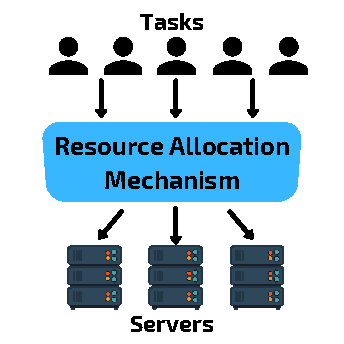
\includegraphics[width=0.6\linewidth]{figures/system_model.pdf}
    \caption{System Model}
    \label{fig:system_model}
\end{figure}

\subsection{System model}
A sketch of the system is shown in Fig.~\ref{fig:system_model}. % To do add figure sketch
We assume that in the system there is a set of servers $I = \{1,2,\ldots,\left|I\right|\}$ servers, which could be edge clouds that can be accessed either through cellular base stations or WiFi access points (APs). Servers have different types of resources: storage for the code/data needed to run a task (e.g., measured in GB), computation capacity in terms of CPU cycles per time interval (e.g., measured in FLOP/s), and communication bandwidth to receive the data and to send back the results of the task after execution (e.g., measured in Mbit/s). We assume that the servers are heterogeneous in all their characteristics. More formally, we denote the storage capacity of server $i$ with $S_i$, computation capacity with $W_i$, and the communication capacity with $R_i$.

There is a set $J = \{1,2,\ldots,\left| J \right|\}$ of  different tasks that require service from one of the servers.\footnote{We focus on a single-shot setting in this paper. In practice, an allocation mechanism would repeat the allocation decisions described here over regular time intervals, with longer-running tasks re-appearing on consecutive time intervals. We leave a detailed study of this to future work.}  Every task $j \in J$ has a value $v_j$ that represents the value of running the task to its owner. To run any of these tasks on a server requires storing the appropriate code/data on the same server. These could be, for example, a set of images, videos or CNN layers in identification tasks. The storage size of task $j$ is denoted as $s_j$ with the rate at which the program is transferred to the server being $s^{'}_j$. For a task to be computed successfully, it must fetch and execute instructions on a CPU. We consider the total number of CPU cycles required for the program to be $w_j$, where the rate at which the CPU cycles are assigned to the task per unit of time is $w^{'}_j$. Finally, after the task is run and the results obtained, the latter need to be sent back to the user. The size of the results for task $j$ is denoted with $r_j$, and the rate at which they are sent back to the user is $r^{'}_j$. Every task has its deadline, denoted by $d_j$. This is the maximum time for the task to be completed in order for the user to derive its value. This time includes: the time required to send the data/code to the server, run it on the server, and get back the results. We assume that there is an \emph{all} or \emph{nothing} task execution reward scheme, meaning that for the task value to be awarded the entire task must be run and the results sent back within the deadline.

% SEB: I've removed the pre-emption comment below - I think this is not relevant in the single-shot setting, because all tasks are allocated at once, no?

%The setup we consider in this paper is non-preemptive, i.e., once a task is assigned to a server, it cannot be stopped to admit another task (possibly of higher importance). 
%This is reasonable given that we look at the problem as a single-shot. Considering the dynamic scenario and the cases where preemption is allowed is beyond the scope of this work.   


\subsection{Optimization problem}\label{subsec:optimisation-problem}

Given the aforementioned assumptions, the optimal assignment of tasks to servers and optimal allocation of resources in a server to the tasks assigned to that server is obtained as a solution to the following optimization problem. Here, the decision variables are $x_{i,j} \in \{0,1\}$ (whether to run task $j$ on server $i$) as well as  $s^{'}_j$, $r^{'}_j$ and $w^{'}_j$  (indicating the bandwidth rates for transferring the code, for returning the results and the CPU cycles per unit of time, respectively). 

\begin{align}
    \max & \sum_{\forall j \in J} v_j \left(\sum_{\forall i \in I} x_{i,j}\right)\label{eq:objective}\\
    \mbox{s.t.} \nonumber \\
    & \sum_{\forall j \in J} s_j x_{i,j} \leq S_i, &~ \forall i \in I,\label{eq:server_storage_constraint}\\
    & \sum_{\forall j \in J} w^{'}_j x_{i,j} \leq W_i, &~ \forall i \in I,\label{eq:server_computation_constraint}\\
    & \sum_{\forall j \in J} (r^{'}_j + s^{'}_j) \cdot x_{i,j} \leq R_i, &~ \forall i \in I,\label{eq:server_communication_constraint}\\
    & \frac{s_j}{s^{'}_j} + \frac{w_j}{w^{'}_j} + \frac{r_j}{r^{'}_j} \leq d_j, &~ \forall{j \in J},\label{eq:job_deadline}\\ 
    & 0 \le s^{'}_j \le \infty, &~ \forall{j \in J,}\label{eq:loading_speeds}\\
    & 0 \le w^{'}_j \le \infty, &~ \forall{j \in J,}\label{eq:compute_speeds}\\
    & 0 \le r^{'}_j \le \infty, &~ \forall{j \in J,}\label{eq:sending_speeds}\\
    & \sum_{\forall i \in I} x_{i,j} \leq 1, &~ \forall j \in J,\label{eq:server_job_allocation}\\
    & x_{i,j} \in \{0, 1\}, &~ \forall{i \in I},\forall{j \in J}.\label{eq:job_allocation}
\end{align}

The objective (Eq.\eqref{eq:objective}) is to maximize the total value over all tasks (i.e., the social welfare). Task $j$ will receive the full value $v_j$ only if it is executed entirely and the results are obtained within
the deadline for that task. Constraint (Eq.\eqref{eq:server_storage_constraint}) relates to the finite storage capacity of every server to store code/data for the tasks that are to be run. The finite computation capacity of every server is expressed through Eq.\eqref{eq:server_computation_constraint}, whereas Eq.\eqref{eq:server_communication_constraint} denotes the constraint on the communication capacity of the servers. As can be seen, the communication bandwidth comprises two parts: one part to send the data/code or request to the server, and the other part to get the results back to the user.\footnote{Not that sending and receiving data will not always overlap, but for tractability we assume they deplete a common limited bandwidth resource per time step. This ensures that the bandwidth constraint is always satisfied in practice.} 
Constraint Eq.\eqref{eq:job_deadline} is the deadline  associated with every task, where the total time of the task in the system is the sum of the time to send the request and code/data to the server, time to run the task, and the time it takes the server to send all the results to the user. Note that if a task is not run on any server, this constraint can be satisfied by choosing arbitrarily high bandwidth and CPU rates (without being constrained by the resource limits of any server). The rates at which the code is sent, run and the results are sent back are all positive and finite (Eqs. \eqref{eq:loading_speeds}, 
\eqref{eq:compute_speeds}, \eqref{eq:sending_speeds}). Further, every task is served by at most one server  (Eq.\eqref{eq:server_job_allocation}). Finally, a task is either served or not  (Eq.\eqref{eq:job_allocation}).

\textbf{Complexity:} 
%This optimization problem is a more general case of the 0-1 knapsack problem, known as the multi-dimensional kn which is
%known to be NP-hard~\cite{}. As a result, this is an NP-hard problem.
In the following we show that this optimization problem is NP-hard. 

\begin{theorem}
    The optimization problem \eqref{eq:objective}-\eqref{eq:job_allocation} is NP-hard.
\end{theorem}
\begin{proof}
    The optimization problem without constraint \eqref{eq:job_deadline} is a 0-1 multidimensional knapsack problem~\cite{knapsackproblems_2004}, which is a generalization of a simple 0-1 knapsack problem. The latter is an NP-hard problem~\cite{knapsackproblems_2004}. Given this, it follows that the 0-1 multidimensional knapsack problem is also NP-hard. Since optimization problem \eqref{eq:objective}-\eqref{eq:job_allocation} is a generalization of a 0-1 multidimensional knapsack problem, it follows that it is NP-hard as well. 
\end{proof}

Before we propose our novel allocation mechanisms for the  allocation problem with elastic resources, we briefly outline an example that illustrates why considering this elasticity is important. In this example, there are 12 potential tasks and 3 servers (the exact settings can be found in  Appendix~\ref{app:example_setting} (Table~\ref{table:jobs} for the tasks and Table~\ref{table:servers} for the servers).

Figure~\ref{fig:fixed_resources_speeds} shows the best possible allocation if tasks have fixed resource requirements. The resource speeds were chosen such to  the minimum total resource usage that the task would require from the deadline. Here, 9 of the tasks are run, resulting in a total social welfare of \hl{XXX} due to the limitation of the server's computation and the task requirement not being balanced.

In contrast to this, Figure~\ref{fig:flexible_resources_speeds} depicts the optimal allocation if elastic resources are considered. Here, it is evident that all of the resources are used by the servers whereas the fixed (in figure~\ref{fig:fixed_resources_speeds}) cant do this. In total, the elastic approach manages to schedule all 12 tasks within the resource constraints, achieving a total social welfare of \hl{YYY} (an \hl{XYZ\%} improvement over the fixed approach).

The figures represent resource usage of the servers by the three bars relating to each of this resources (storage, CPU and bandwidth). For each task that is allocated to the server, the percentage of the resource's used is bar size. Then, for the tasks that are assigned to corresponding servers, the percentage of used resources are also depicted.

\begin{figure}[th]
    \centering
    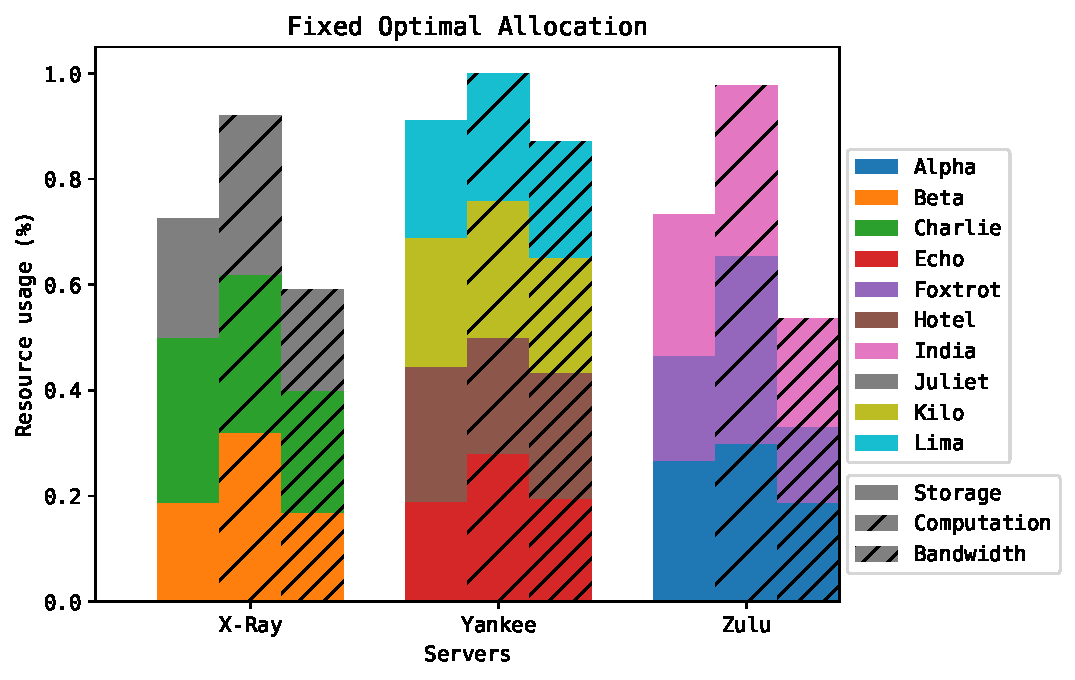
\includegraphics[width=\linewidth]{figures/fixed_optimal_allocation.pdf}
    \caption{Optimal solution with fixed resources. Due to not being able to balance out the resources, bottlenecks on the server 1 and 2's computation have occurred}
    \label{fig:fixed_resources_speeds}
\end{figure}

\begin{figure}[th]
    \centering
    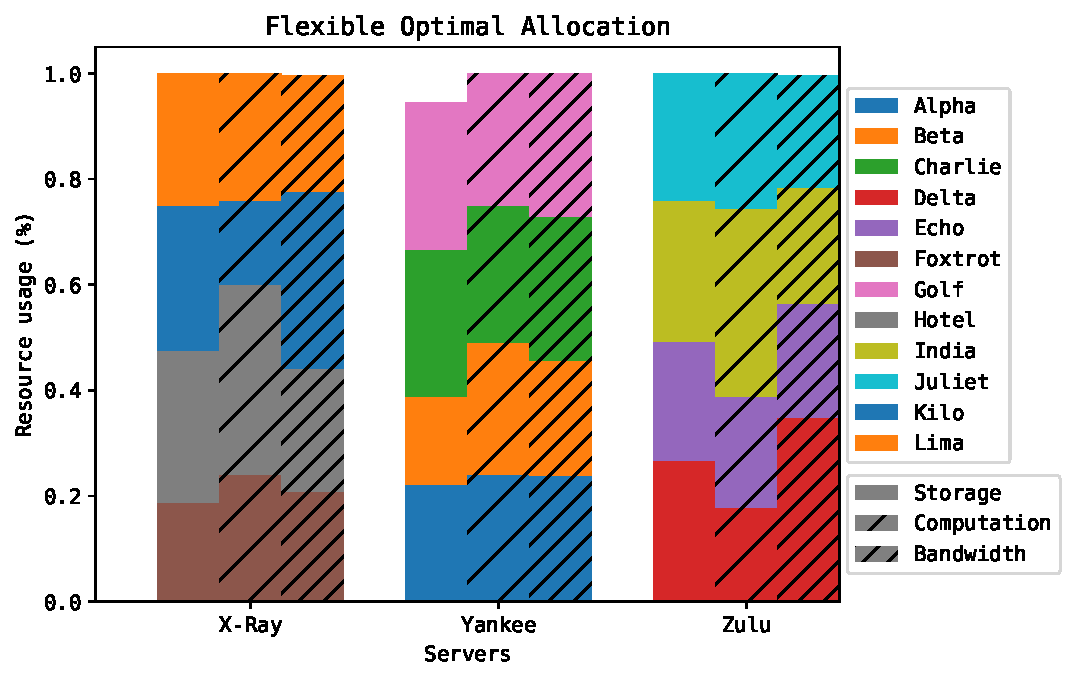
\includegraphics[width=\linewidth]{figures/flexible_optimal_allocation.pdf}
    \caption{Optimal solution with elastic resources. Compared to the fixed allocation, the elastic allocation is able to fully use all of its resources}
    \label{fig:flexible_resources_speeds}
\end{figure}

%An example of the impact of using flexible resource speeds is shown in Figs.  and \ref{fig:fixed_resources_speeds}.
%In this model, the optimal fixed resource allocation means that only 9 of the 12 tasks are able to be allocated with social welfare of XXX. % What is the value? 
%As opposed to this, flexible resource allocation can allocate all of the tasks with social welfare of XXX. % Don't forget the value 
%The task and server attributes are given in Appendix \ref{app:example_setting} (Table \ref{table:jobs} for the tasks and Table \ref{table:servers} for the servers). 
%Fig.~\ref{fig:flexible_resources_speeds} contains a grouping for each of the server with the three bars relating to each of the resources (storage, CPU and bandwidth). 
%Then for each task that is allocated to the server, the percentage of the resource's used is bar size. 
%Then, for the tasks that are assigned to corresponding servers, the percentage of used resources are also depicted.

\section{Flexible Resource Allocation Mechanisms}\label{sec:flexible-resource-allocation-mechanisms}
%Algorithms presented in \cite{Nip2017} allow for solving flexible knapsack problems with linear constraints to maximise the social welfare.
%However, our problem case contains non-linear constraints and the algorithm's time complexity is $O(J^{I+J})$ for our problem case; where $J$ and $I$ are the 
%number of tasks and servers respectively. This makes using the algorithm impractical as the solve time could exceed the deadline for some tasks.
%Previous research hasn't considered any auction mechanisms and as servers would wish to be paid for the use of their resources, we have also
%proposed two auction mechanisms.

In this section, we propose several mechanisms for solving the resource allocation problem with elastic resources. First, we discuss a centralized greedy algorithm (detailed in Section~\ref{subsec:greedy-mechanism}) with a $\frac{1}{\left|J\right|}$ performance guarantee and polynomial run-time. Then, we consider settings where task users are self-interested and may either report their task values and requirements strategically or may wish to limit the information they reveal to the mechanism. To deal with such cases, we propose two auction-based  mechanisms, one of which can be executed in a decentralized manner (in Sections~\ref{subsec:critical-value-auction} and \ref{subsec:decentralised-iterative-auction}). 

\subsection{Greedy Mechanism}\label{subsec:greedy-mechanism}
As solving the allocation problem with elastic resources is NP-hard, we here propose a greedy algorithm (algorithm \ref{alg:greedy_mechanism}) that considers tasks individually, based on an appropriate prioritisation function.
%Due to the flexible nature of resources, in order to optimally allocate them, the problem in section~\ref{subsec:optimisation-problem} must be solved. This is infeasible due to the constraints discussed above. Therefore, when allocating for a task, a prediction must be made based on the current resource availability. In order to maximise the social welfare, the most valuable tasks take allocation priority.

More specifically, the greedy algorithm does this in two stages; the first sorts the tasks and the second allocates them to servers. A value density function is applied to each of the task based on its attributes: value, required resources and deadlines. Stage one uses this function to sort the list of tasks. The second stage then iterates through the tasks in the given order, applying two heuristics to each task: one to select the server and another to allocate resources. The first of these heuristics, called the server selection heuristic, works by checking if a server could run the task if all of it's resources were to be used forfill the deadline constraint (eq~\ref{eq:job_deadline}) then calculating how good it would be for the job to be allocated to the server. The second heuristic, called the resource allocation heuristic, finds the best permutations of resources to minimum a formula, i.e. the total percentage of server resources used by the task. 

In this paper we prove that the lower bound of the algorithm is $\frac{1}{n}$ where $n$ is the number of jobs using the value of a task as the value density function and using any feasible server selection and resource allocation heuristic. However we found that the task value heuristic is not the best heuristic as it doesn't consider the effect of the deadline or resource used for a job. Therefore we recommend using the following heuristic $\frac{v_j \cdot (s_j + w_j + r_j)}{d_j}$, but do not present a proof for it being analytically better than the value heuristic. For the server selection heuristic we recommend $argmin_{\forall i \in I} S^{'}_i + W^{'}_i + R^{'}_i$ where $S^{'}_i$, $W^{'}_i$, $R^{'}_i$ is the server available of it's resources storage, computation and bandwidth respectively. While for the resource allocation heuristic we recommend $min \frac{W^{'}_i}{w^{'}_j} + \frac{R^{'}_i}{s^{'}_j + r^{'}_j}$ where $s^{'}_j$, $w^{'}_j$ and $r^{'}_j$ adhere to the deadline constraint (eq~\ref{eq:job_deadline}). 

%\subsubsection{Lower bound of greedy mechanism}
\begin{theorem}
    The lower bound of the greedy mechanism is $\frac{1}{n}$ of the optimal social welfare
\end{theorem}
\begin{proof}
    Taking the value of a task as the value density function, the first task allocated will have a value of at least $\frac{1}{n}$ total values of all jobs. As the allocation of resources for a task is not optimal, allocation of subsequent tasks is not guaranteed. Therefore, as the optimal social welfare must be the total values of all jobs or lower then the lower bound of the mechanism must be $\frac{1}{n}$ of the optimal social welfare. 
\end{proof} 
% \begin{conjecture}
%    We conjecture that there is no better lower bound for a fully polynomial time approximation scheme than $\frac{1}{n}$ of optimal .
% \end{conjecture}

In figure~\ref{fig:greedy_allocation}, an example allocation using the algorithm is shown using the model from appendix \ref{app:example_setting}. The algorithm uses the recommend heuristic proposed above and allows for 11 of the 12 tasks to be allocated achieving \hl{XX}\% of the flexible optimal in figure~\ref{fig:flexible_resources_speeds}.  
\todo[inline]{Explain what can be seen in that figure.}

\begin{figure}[H]
    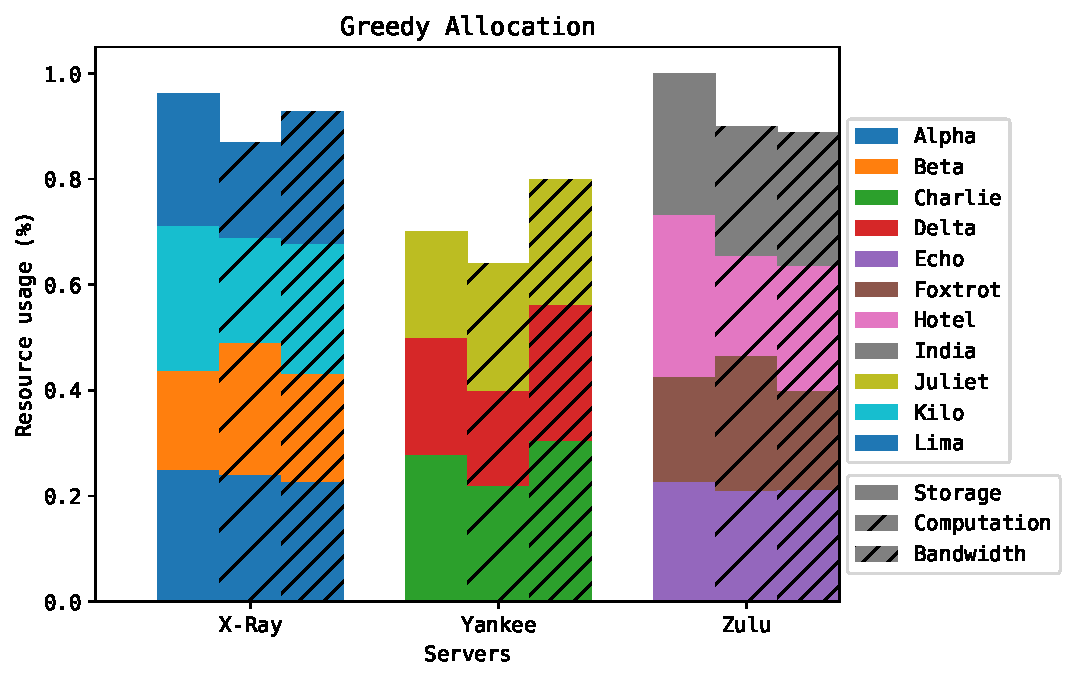
\includegraphics[width=\linewidth]{figures/greedy_allocation.pdf}
    \caption{Example Greedy allocation using model from appendix \ref{app:example_setting}}
    \label{fig:greedy_allocation}
\end{figure}

\begin{algorithm}[]
    \caption{Greedy Mechanism}
    \label{alg:greedy_mechanism}
    \begin{algorithmic}
        \REQUIRE $J$ is the set of tasks and $I$ is the set of servers
        \REQUIRE $S^{'}_i$, $W^{'}_i$ and $R^{'}_i$ is the available resources (storage, computation and bandwidth respectively) for a server $i$. 
        \REQUIRE $\alpha(j)$ is the value density function of a task
        \REQUIRE $\beta(j, I)$ is the server selection function of a task and set of servers returning the best server, 
        or $\emptyset$ if the task is not able to be run on any server
        \REQUIRE $\gamma(j, i)$ is the resource allocation function of a task and server returning the loading, compute and sending speeds
        \REQUIRE $sort(X, f)$ is a function that returns a sorted list of elements in descending order, based on a set of elements and a function for comparing elements
        \STATE{$J^{'} \leftarrow sort(J, \alpha)$}
        \FORALL{$j \in J^{'}$}
            \STATE{$i \leftarrow \beta(j, I)$}
            \IF{$i \neq \emptyset$}
                \STATE{$s^{'}_j, w^{'}_j, r^{'}_j \leftarrow \gamma(j, i)$}
                \STATE{$x_{i,j} \leftarrow 1$}
            \ENDIF
        \ENDFOR
    \end{algorithmic}
\end{algorithm}

%\subsubsection{Time complexity of greedy mechanism}\label{subsubsec:greedy_time_complexity}
\begin{theorem}
    The time complexity of the greedy algorithm is $O(\left|J\right| \left|I\right|)$, where $\left|J\right|$ is the number of tasks and $\left|I\right|$ is the number of servers.
    Assuming that the value density and resource allocation heuristics have constant time complexity and the server selection function is $O(\left|I\right|)$.
\end{theorem}
\begin{proof}
    The time complexity of the stage 1 of the mechanism is $O(\left|J\right| \log(\left|J\right|))$ due to sorting the tasks and stage 2 has complexity $O(\left|J\right| \left|I\right|)$ due to looping over all of the tasks and applying the server selection and resource allocation heuristics. Therefore the overall time complexity is $O(\left|J\right| \left|I\right| + \left|J\right| \log(\left|J\right|) = O(\left|J\right| \left|I\right|)$.  
\end{proof}

\subsection{Critical Value Auction}\label{subsec:critical-value-auction}
Due to the problem case being non-cooperative, if the greedy mechanism was used to allocate resources such that the value is the price paid. This is open to manipulation and misreporting of task attributes like the value, deadline or resource requirements. Therefore in this section we propose an auction that is weakly-dominant for tasks to truthfully report it attributes. 

Single-Parameter domain auctions are extensively studied in mechanism design~\cite{nisan2007algorithmic_228} and are used where an agent's valuation function can be represented as single value. The task price is calculated by finding the task's value such that if the value were any smaller, the task could not be allocated. This value is called the critical value. This has been shown to be a strategyproof~\cite{nisan2007algorithmic_229_230} (weakly-dominant incentive compatible) auction so it is a weakly-dominant strategy for a task to honestly reveal its value. 

The auction is implemented using the greedy mechanism from section~\ref{subsec:greedy-mechanism} to find an allocation of tasks using the reported value. Then for each task allocated, the last position in the ordered the task list such that the task would still allocated is found. The critical value of the task is then equal to the inverse of the value density function where the density is the density of the next task in the list after that position.

In order that the auction is strategyproof, the value density function is required to be monotonic. Meaning that misreporting of task attributes will result in the value density decreasing. We propose the value density function of $\frac{v_j d_j}{s_j + w_j + r_j}$ however any function that is monotonic for the combination of the resource requirement variables on the denominator is valid. 
\begin{theorem}
    The value density function $\frac{v_j d_j}{\alpha(s_j, w_j, r_j)}$ is monotonic for task $j$
    Assuming the function $\alpha(s_j, w_j, r_j)$ is monotonic
\end{theorem}
\begin{proof}
    In order to misreport the task private value and deadline must be less than the true value. The opposite is true for the required resources (storage, compute and result data) with the misreported value being greater than the true value. Therefore the $\alpha$ function will increase as the resource requirements increase as well, meaning that density will decrease. 
\end{proof}

\subsection{Decentralised Iterative Auction}\label{subsec:decentralised-iterative-auction}
VCG (Vickrey-Clark-Grove) auction \cite{vickrey} \cite{clarke} \cite{groves} is proven to be economically efficient, budget balanced and incentive compatible. A task's price is found by the difference of the social welfare for when the task exists compared to the social welfare when the task doesn't exist. Our auction uses the same principle for pricing by finding the difference between the current server revenue and the revenue when the task is allocated (at £0).

The auction iteratively lets a task advertise its requirements to all of the servers who respond with their price for the task. This price is equal to the server's current revenue minus the solution to the the problem in section~\ref{subsubsec:decentralised_iterative_problem} plus a small value called the price change variable. Being the reverse of the VCG mechanism, such that the price is found for when the task exists rather than when it doesn't exist. The price change variable allows for the increase in the revenue of the server and is can be chosen by the server. Once all of the server have responded, the task can compare the minimum server price to its private value. If the price is less then the task will accept the servers with the minimum price offer, otherwise the task will stop looking as the price for the task to run on any server is greater than its reserve price. 

To find the optimal revenue for a server $m$ given a new task $p$ and set of currently allocated tasks $N$ has a similar formulation to section~\ref{subsec:optimisation-problem}. With an additional variable is considered, a task's price being $p_n$ for task $n$.

\subsubsection{Server problem case}\label{subsubsec:decentralised_iterative_problem}
\begin{align}
    \max & \sum_{\forall n \in N} p_n x_n\label{eq:dia_objective}\\
    \mbox{s.t.} \\
    & \sum_{\forall n \in N} s_n x_n + s_p \leq S_m,\label{eq:dia_server_storage_constraint}\\
    & \sum_{\forall n \in N} w^{'}_n x_n + w_p \leq W_m, \label{eq:dia_server_computation_constraint}\\
    & \sum_{\forall n \in N} (r^{'}_n + s^{'}_n) \cdot x_n + (r^{'}_p + s^{'}_p) \leq R_m, \label{eq:dia_server_communication_constraint}\\
    & \frac{s_n}{s^{'}_n} + \frac{w_n}{w^{'}_n} + \frac{r_n}{r^{'}_n} \leq d_n, &~ \forall n \in N \cup \{p\}, \label{eq:dia_job_deadline}\\
    & 0 \le s^{'}_n \le \infty, &~ \forall{n \in N \cup \{p\}} \label{eq:dia_loading_speeds}\\
    & 0 \le w^{'}_n \le \infty, &~ \forall{n \in N \cup \{p\}} \label{eq:dia_compute_speeds}\\
    & 0 \le r^{'}_n \le \infty, &~ \forall{n \in N \cup \{p\}} \label{eq:dia_sending_speeds}\\
    & x_n \in \{0,1\}, &~ \forall{n \in N} \label{eq:dia_job_allocation}
\end{align}

The objective (Eq.\eqref{eq:dia_objective}) is to maximize the price of all tasks (not including the new task as the price is zero). The server resource capacity constraints are similar to the constraints in the standard model set out in section~\ref{subsec:optimisation-problem} however with the assumption that the task $k$ is running so there is no need to consider if the task is running or not. The deadline and non-negative resource speeds constraints (\ref{eq:job_deadline}, \ref{eq:loading_speeds}, \ref{eq:compute_speeds} and \ref{eq:sending_speeds}) are all the same equation with the new task included with all of the other tasks. The equation to check that a task is only allocated to a single server is not included as only server $i$ considers the task $k$'s price. 

In auction theory, four properties are considered: Incentive compatible, budget balanced, economically efficient and individual rationality.
\begin{itemize}
    \item Budget balanced - Since the auction is run without an auctioneer, this allows for the auction to be run 
    in a decentralised way resulting in no ''middlemen'' taking some money so all revenue goes straight to the servers from the tasks 
    \item Individually Rational - As the server need to confirm with the task if it is willing to pay an amount to be allocated,
    the task can check this against its secret reserved price preventing the task from ever paying more than it is willing
    \item Incentive Compatible - Misreporting can give a task as if the task can predict the allocation of resources from server to tasks then 
     tasks can misreport so to be allocate to a certain server that otherwise would result in the task being unallocated. 
     An example of this happening is in appendix \ref{app:incentive_compatible_example}
    \item Economic efficiency - At the begin then task are almost randomly assigned in till server become full and require kicking tasks off,
    this means that allocation can fall into a local price maxima meaning that the server will sometime not be 100\% economically 
    efficient.
\end{itemize}

\begin{algorithm}[H]
    \caption{Decentralised Iterative Auction}
    \label{alg:dia}
    \begin{algorithmic}
        \REQUIRE $I$ is the set of servers
        \REQUIRE $J$ is the set of unallocated tasks, which initial is the set of all tasks to be allocated
        \REQUIRE $P(i, k)$ is solution to the problem in section~\ref{subsubsec:decentralised_iterative_problem}
        using the server $i$ and new task $k$. 
        The server's current tasks is known to itself and its current revenue from tasks so not passed as arguments. 
        \REQUIRE $R(i, k)$ is a function returning the list of tasks not able to run if task $k$ is allocated to server $i$
        \REQUIRE $\leftarrow_R$ will randomly select an element from a set
        \WHILE{$|J| > 0$}
            \STATE{$j \leftarrow_R J$}
            \STATE{$p, i \leftarrow argmin_{i \in I} P(i, j)$}
            \IF{$p \leq v_j$}
                \STATE{$p_j \leftarrow p$}
                \STATE{$x_{i, j} \leftarrow 1$}
                \FORALL{$j^{'} \in R(i, j)$}
                    \STATE{$x_{i, j^{'}} \leftarrow 0$}
                    \STATE{$p_j^{'} \leftarrow 0$}
                    \STATE{$J \leftarrow J \cup j^{'}$}
                \ENDFOR
            \ENDIF
            \STATE{$J \leftarrow J \setminus \{j\}$}
        \ENDWHILE
    \end{algorithmic}
\end{algorithm}

The algorithm \ref{alg:dia} is a centralised version of the decentralised iterative auction. It works through iteratively checking a currently unallocated job to find the price if the job was currently allocated on a server. This is done through first solving the program in section \ref{subsubsec:decentralised_iterative_problem} which calculates the new revenue if the task was forced to be allocated with a price of zero. The task price is equal to the current server revenue $-$ new revenue with the task allocated $+$ a price change variable to increase the revenue of the server. The minimum price returned by $P(i, k)$ is then compared to the job's maximum reserve price (that would be private in the equivalent decentralised algorithm) to confirm if the job is willing to pay at that price. If the job is willing then the job is allocated to the minimum price server and the job price set to the agreed price. However in the process of allocating a job then the currently allocated jobs on the server could be unallocated so these jobs allocation's and price's are reset then appended to the set of unallocated jobs. 

\subsection{Attributes of proposed algorithms}
In table~\ref{tab:attributes_algorithms}, the important attributes for the proposed algorithm 
\begin{table}[H]
    \centering
    \begin{tabular}{|p{2.2cm}|p{1.5cm}|p{1.5cm}|p{1.5cm}|}
        \hline
        Attribute & GM & CVA & DIA \\ \hline \hline
        Truthfulness & & weakly-dominant & Not \\ \hline 
        Optimality & Close & Close & Close to optimal \\ \hline 
        Scalability & High & Medium & Low \\ \hline 
        Information requirements from users & All & All & Not value \\ \hline 
        Communication over heads & Low & Low & High \\ \hline 
        Decentralisation & No & No & Yes \\ \hline 
    \end{tabular}
    \caption{Attributes of the proposed algorithms: Greedy mechanism (GM), Critical Value auction(CVA) and Decentralised Iterative auction (DIA)}
    \label{tab:attributes_algorithms}
\end{table}

\section{Empirical Evaluation}\label{sec:empirical-evaluation}
To test the algorithm shown in section~\ref{sec:flexible-resource-allocation-mechanisms}, a mixture of synthetic models
and real world data is used to generate our tasks and servers.
The synthetic model are generated randomly by Gaussian distribution of the attributes for the tasks and servers 
by selecting a mean and standard deviation.
The real world data is from a Google cluster data from 2011 that contain the requested CPU cores, memory, 
local disk space, priority by users and the total execution time of the program.

\subsection{Greedy mechanism testing}\label{subsec:greedy-mechanism-testing}
To compare the result of the greedy algorithm in figure~\ref{fig:greedy_shortened_sum_value}, the optimal solution 
was found by using a constraint problem solver and a relaxed variation of the problem was used where the optimal
solution could not be found. The relaxed problem considered where all server were combined together into a ''super''
server creating an upper bound on the problem. 

\begin{figure}[H]
    
\includegraphics[width=\linewidth]{figures/greedy_algorithm.eps}
    \caption{Sum Value results for Optimal, Relaxed and Greedy Algorithms.}
    \label{fig:greedy_shortened_sum_value}
\end{figure}

Figure~\ref{fig:greedy_shortened_sum_value} shows that average the greedy algorithm will be over 90\% efficient in 
its allocation as the optimal solution with a tight confidence interval. Which is true for models with a large and small 
number of tasks and servers making it stable. 
The heuristics used for the greedy algorithm used are: the task value divided by total resource requirements as value density,
server selected with the minimum available total resources and the resource allocation based on the minimum percentage of the 
server's resources used. 

\subsection{Auction mechanisms testing}\label{subsec:auctiom-mechanisms-testing}
To test our two auction mechanisms, we have compared the results to a VCG auction and a fixed VCG auction where the task speeds
are fixed before allocation.
\begin{figure}[H]
    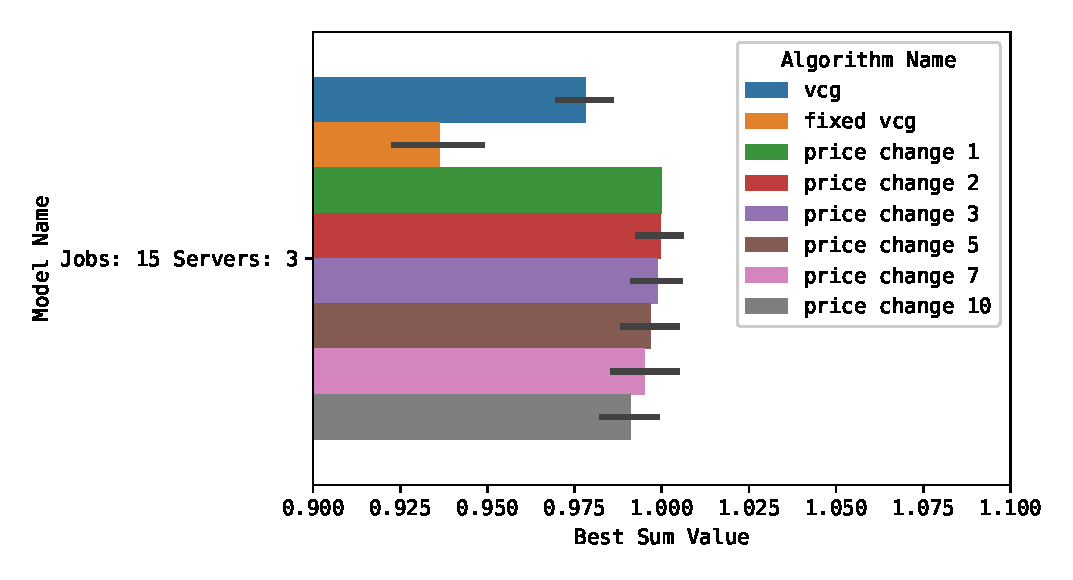
\includegraphics[width=\linewidth]{figures/price_change_sum_value.eps}
    \caption{The sum value of the tasks using different algorithms.}
    \label{fig:price_change}
\end{figure}
In figure~\ref{fig:price_change} this shows that the price change variable does not have a significant impact on the 
social welfare of the system. % Todo add more. 

An important factor of the decentralised iterative auction is the number of rounds required till the algorithm converges
to the optimal pricing as this is proportional to the time for the auction to complete. 
In figure~\ref{fig:iterative_round_iterative_heapmap} and \ref{fig:iterative_round_money_heapmap} investigate the affect of 
the price change and an initial task pricing heuristic on the total revenue and the number of rounds required for the 
auction to completed. 
The heapmap clearly shows that the price change variable has a huge effect on the average number of rounds in an auction
where the initial cost has a negligible effect on the number of rounds. 
However the effect of have less rounds does not have as large an effect on the total revenue of the servers meaning that 
the tradeoff of rounds to revenue does not matter to a large degree. 
% The heapmap graph are not true as the initial cost argument was bugged with this current data. This is being run now to get new data. Therefore To do again later. 
\begin{figure}[H]
    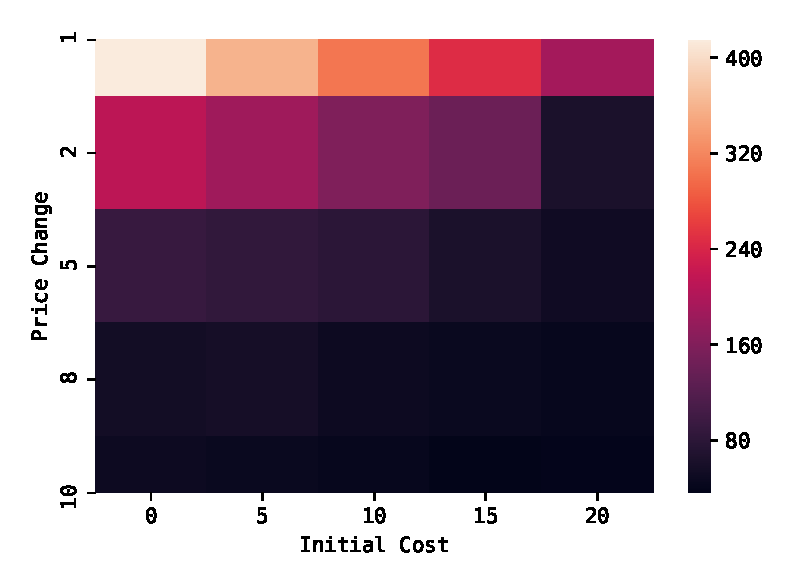
\includegraphics[width=\linewidth]{figures/iterative_round_number_heatmap.eps}
    \caption{The number of rounds that on average that are required to price equilibrium compared to the number required for the auction with an initial cost of 0 and price change of 1.}
    \label{fig:iterative_round_iterative_heapmap}
\end{figure}
\begin{figure}[H]
    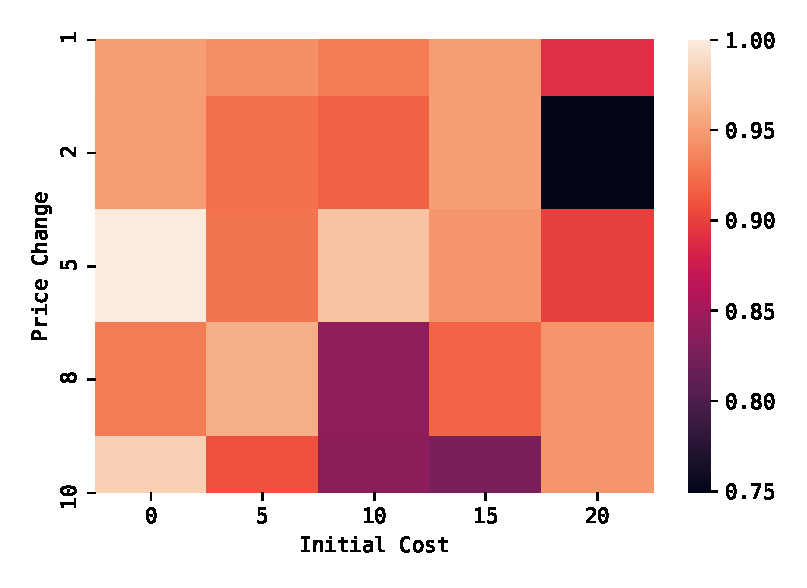
\includegraphics[width=\linewidth]{figures/iterative_money_heatmap.eps}
    \caption{The percentage difference in revenue that on average compared to the revenue gain in the auction with an initial cost of 0 and price change of 1.}
    \label{fig:iterative_round_money_heapmap}
\end{figure}

As shown in section~\ref{subsec:decentralised-iterative-auction}, the decentralised iterative auction is not a truthful
auction meaning that lying on the resources required can advantage some users. 
In figure~\ref{fig:auction-mutation}, tasks are compared with the price they are required to pay when truthfully reported, 
in orange, while the a mutated task in the same model is shown in blue. In almost all cases, the task is required to pay more 
money to be run than compared to when truthfully reported however in the anomalous cases, these are due to originally not being 
allocated and in the mutated case the task is then allowed to be run. 
However this can occur if allocation is in a local maximum and is not in the global pricing maxima which means that 
inefficient allocation can occur. % To prove
\begin{figure}[H]
    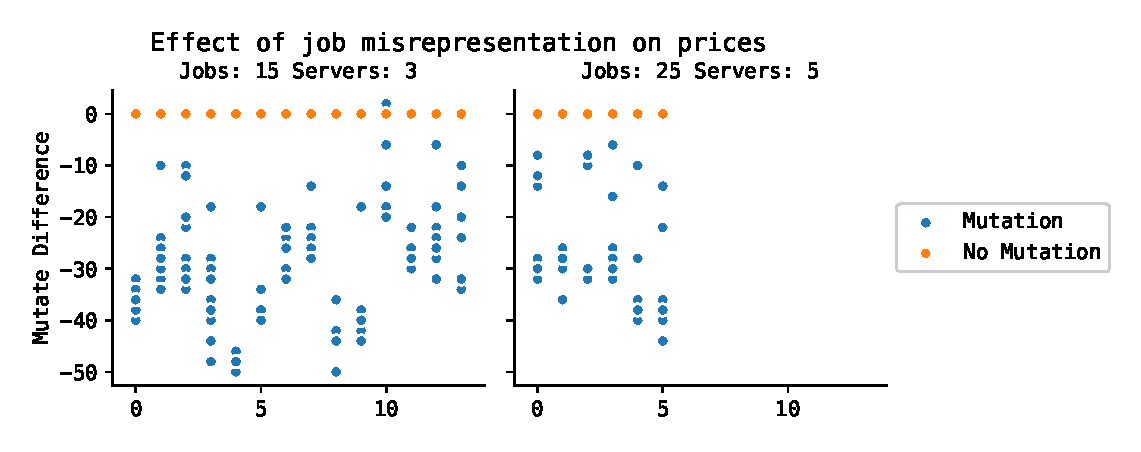
\includegraphics[width=\linewidth]{figures/mutate_auction.eps}
    \caption{Measuring the difference in price when the task is incorrectly reported.}
    \label{fig:auction-mutation}
\end{figure}

% To do: Add the critical value analysis, more greed analysis, non uniform price change analysis

\section{Conclusions}\label{sec:conclusions-and-future-work}
In this paper we have looked at the problem of optimally assigning tasks of different values to servers, and to optimally allocate the elastic resources (computation power and communication bandwidth) to the tasks within the servers. We have shown that the problem is NP-hard. Then, we have proposed three mechanisms for solving this problem. The first one is a greedy mechanism to maximise the social welfare of the tasks where the task value is revealed. The other two are auction-based mechanisms. The first of them is a single-parameter domain- based auction that uses the greedy mechanism to calculate the critical value of the allocated tasks and requires that each task reveals its value. This is a weakly-dominant incentive compatible auction mechanism. Finally, the last auction mechanism is a decentralised iterative auction that doesn't require each task to reveal its task value. Instead, it calculates a reverse VCG price for the task to run on a server. 

In future work, we plan to consider the dynamic scenario, where tasks arrive and depart from the system over time, and to also consider the case where task preemption is allowed. 

\appendix

\section{Example Setting}\label{app:example_setting}
\begin{table}[]
    \begin{tabular}{|c||c|c|c|} 
        \hline
        Name & $S_i$ & $W_i$ & $R_i$ \\ [0.5ex] \hline\hline
        Server 1 & 400 & 100 & 220 \\ \hline
        Server 2 & 450 & 100 & 210 \\ \hline
        Server 3 & 375 & 90  & 250 \\ \hline
    \end{tabular}
    \caption{\textbf{Servers} - Table of server attributes\\}
    \label{table:servers}
\end{table}

\begin{table}[]
    \begin{tabular}{|c||c|c|c|c|c||c|c|c|} 
        \hline
        Name & $v_j$ & $s_j$ & $w_j$ & $r_j$ & $d_j$ \\ [0.5ex] \hline\hline
        Task 1  & 100 & 100 & 100 & 50 & 10 & 30 & 24 & 20 \\ \hline
        Task 2  & 90  & 75  & 125 & 40 & 10 & 30 & 25 & 16 \\ \hline
        Task 3  & 110 & 125 & 110 & 45 & 10 & 36 & 26 & 21 \\ \hline
        Task 4  & 75  & 100 & 75  & 60 & 10 & 23 & 16 & 64 \\ \hline
        Task 5  & 125 & 85  & 90  & 55 & 10 & 34 & 19 & 20 \\ \hline
        Task 6  & 100 & 75  & 120 & 40 & 10 & 25 & 24 & 21 \\ \hline
        Task 7  & 80  & 125 & 100 & 50 & 10 & 38 & 25 & 19 \\ \hline
        Task 8  & 110 & 115 & 75  & 55 & 10 & 37 & 36 & 14 \\ \hline
        Task 9  & 120 & 100 & 110 & 60 & 10 & 40 & 32 & 15 \\ \hline
        Task 10 & 90  & 90  & 120 & 40 & 10 & 32 & 23 & 21 \\ \hline
        Task 11 & 100 & 110 & 90  & 45 & 10 & 34 & 16 & 40 \\ \hline
        Task 12 & 100 & 100 & 80  & 55 & 10 & 25 & 24 & 23 \\ \hline
    \end{tabular}
    \caption{\textbf{Tasks} - Table of task attributes, the columns for resource speeds ($s^{'}_j$, $w^{'}_j$,
    $r^{'}_j$) is for fixed speeds which the flexible allocation does not take into account.}
    \label{table:jobs}
\end{table}

\section{Incentive Compatible Example}\label{app:incentive_compatible_example}
Using tables \ref{table:ic_task_attributes} and \ref{table:ic_servers_attributes} as the task and server attributes. Normally the following
allocation could occur, with price change of \textsterling 2 for both servers.
\begin{itemize}
    \item Task 1 is put on server 1 for \textsterling 2 with resource speeds $s^{'} = 1, w^{'} = 1, r^{'} = 1$
    \item Task 2 is put on server 2 for \textsterling 2 with resource speeds $s^{'} = 1, w^{'} = 1, r^{'} = 1$
    \item Task 3 is put on server 1 for \textsterling 4 with resource speeds $s^{'} = 1, w^{'} = 2, r^{'} = 2$
\end{itemize}

If Task 1 misreports it's required storage as 2 then this would allow task 1 to now get allocated where before it wasn't.
\begin{itemize}
    \item Task 1 is put on server 2 for \textsterling 2 with resource speeds $s^{'} = 2, w^{'} = 1, r^{'} = 1$ as it cant fit on server 1 with a storage requirement of 2
    \item Task 2 is put on server 1 for \textsterling 2 with resource speeds $s^{'} = 1, w^{'} = 1, r^{'} = 1$
    \item Task 3 is put on server 1 for \textsterling 4 with 
    
\end{itemize}

\begin{table}[]
    \begin{tabular}{|c||c|c|c|} 
        \hline
        Name & $S_i$ & $W_i$ & $R_i$ \\ [0.5ex] \hline\hline
        Server 1 & 1 & 2 & 3 \\ \hline
        Server 2 & 2 & 2 & 3 \\ \hline
    \end{tabular}
    \caption{\textbf{Servers} - Table of server attributes\\}
    \label{table:ic_servers_attributes}
\end{table}

\begin{table}[]
    \begin{tabular}{|c||c|c|c|c|c|} 
        \hline
        Name & $v_j$ & $s_j$ & $w_j$ & $r_j$ & $d_j$ \\ [0.5ex] \hline\hline
        Task 1 & 3 & 1 & 1 & 1 & 3 \\ \hline
        Task 2 & 3 & 1 & 1 & 1 & 3 \\ \hline
        Task 3 & 5 & 1 & 2 & 2 & 3 \\ \hline
    \end{tabular}
    \caption{\textbf{tasks} - Table of task attributes.}
    \label{table:ic_task_attributes}
\end{table}

%%%%%%%%%%%%%%%%%%%%%%%%%%%%%%%%%%%%%%%%%%%%%%%%%%%%%%%%%%%%%%%%%%%%%%%%%%%%%%%%%%%%%%%%%%%%%%%%%%%%%%%%%
%% bibliography: see CFP for number of permitted pages

\bibliographystyle{ACM-Reference-Format}  % do not change this line!
\bibliography{bibliography}  % put name of your .bib file here

\end{document}
